\chapter*{Templates to copy from}

You can just keep this file, use it to copy templates from, and delete it after you're done with everything.





\section*{Figure}

\begin{figure}[H]
    \centering
    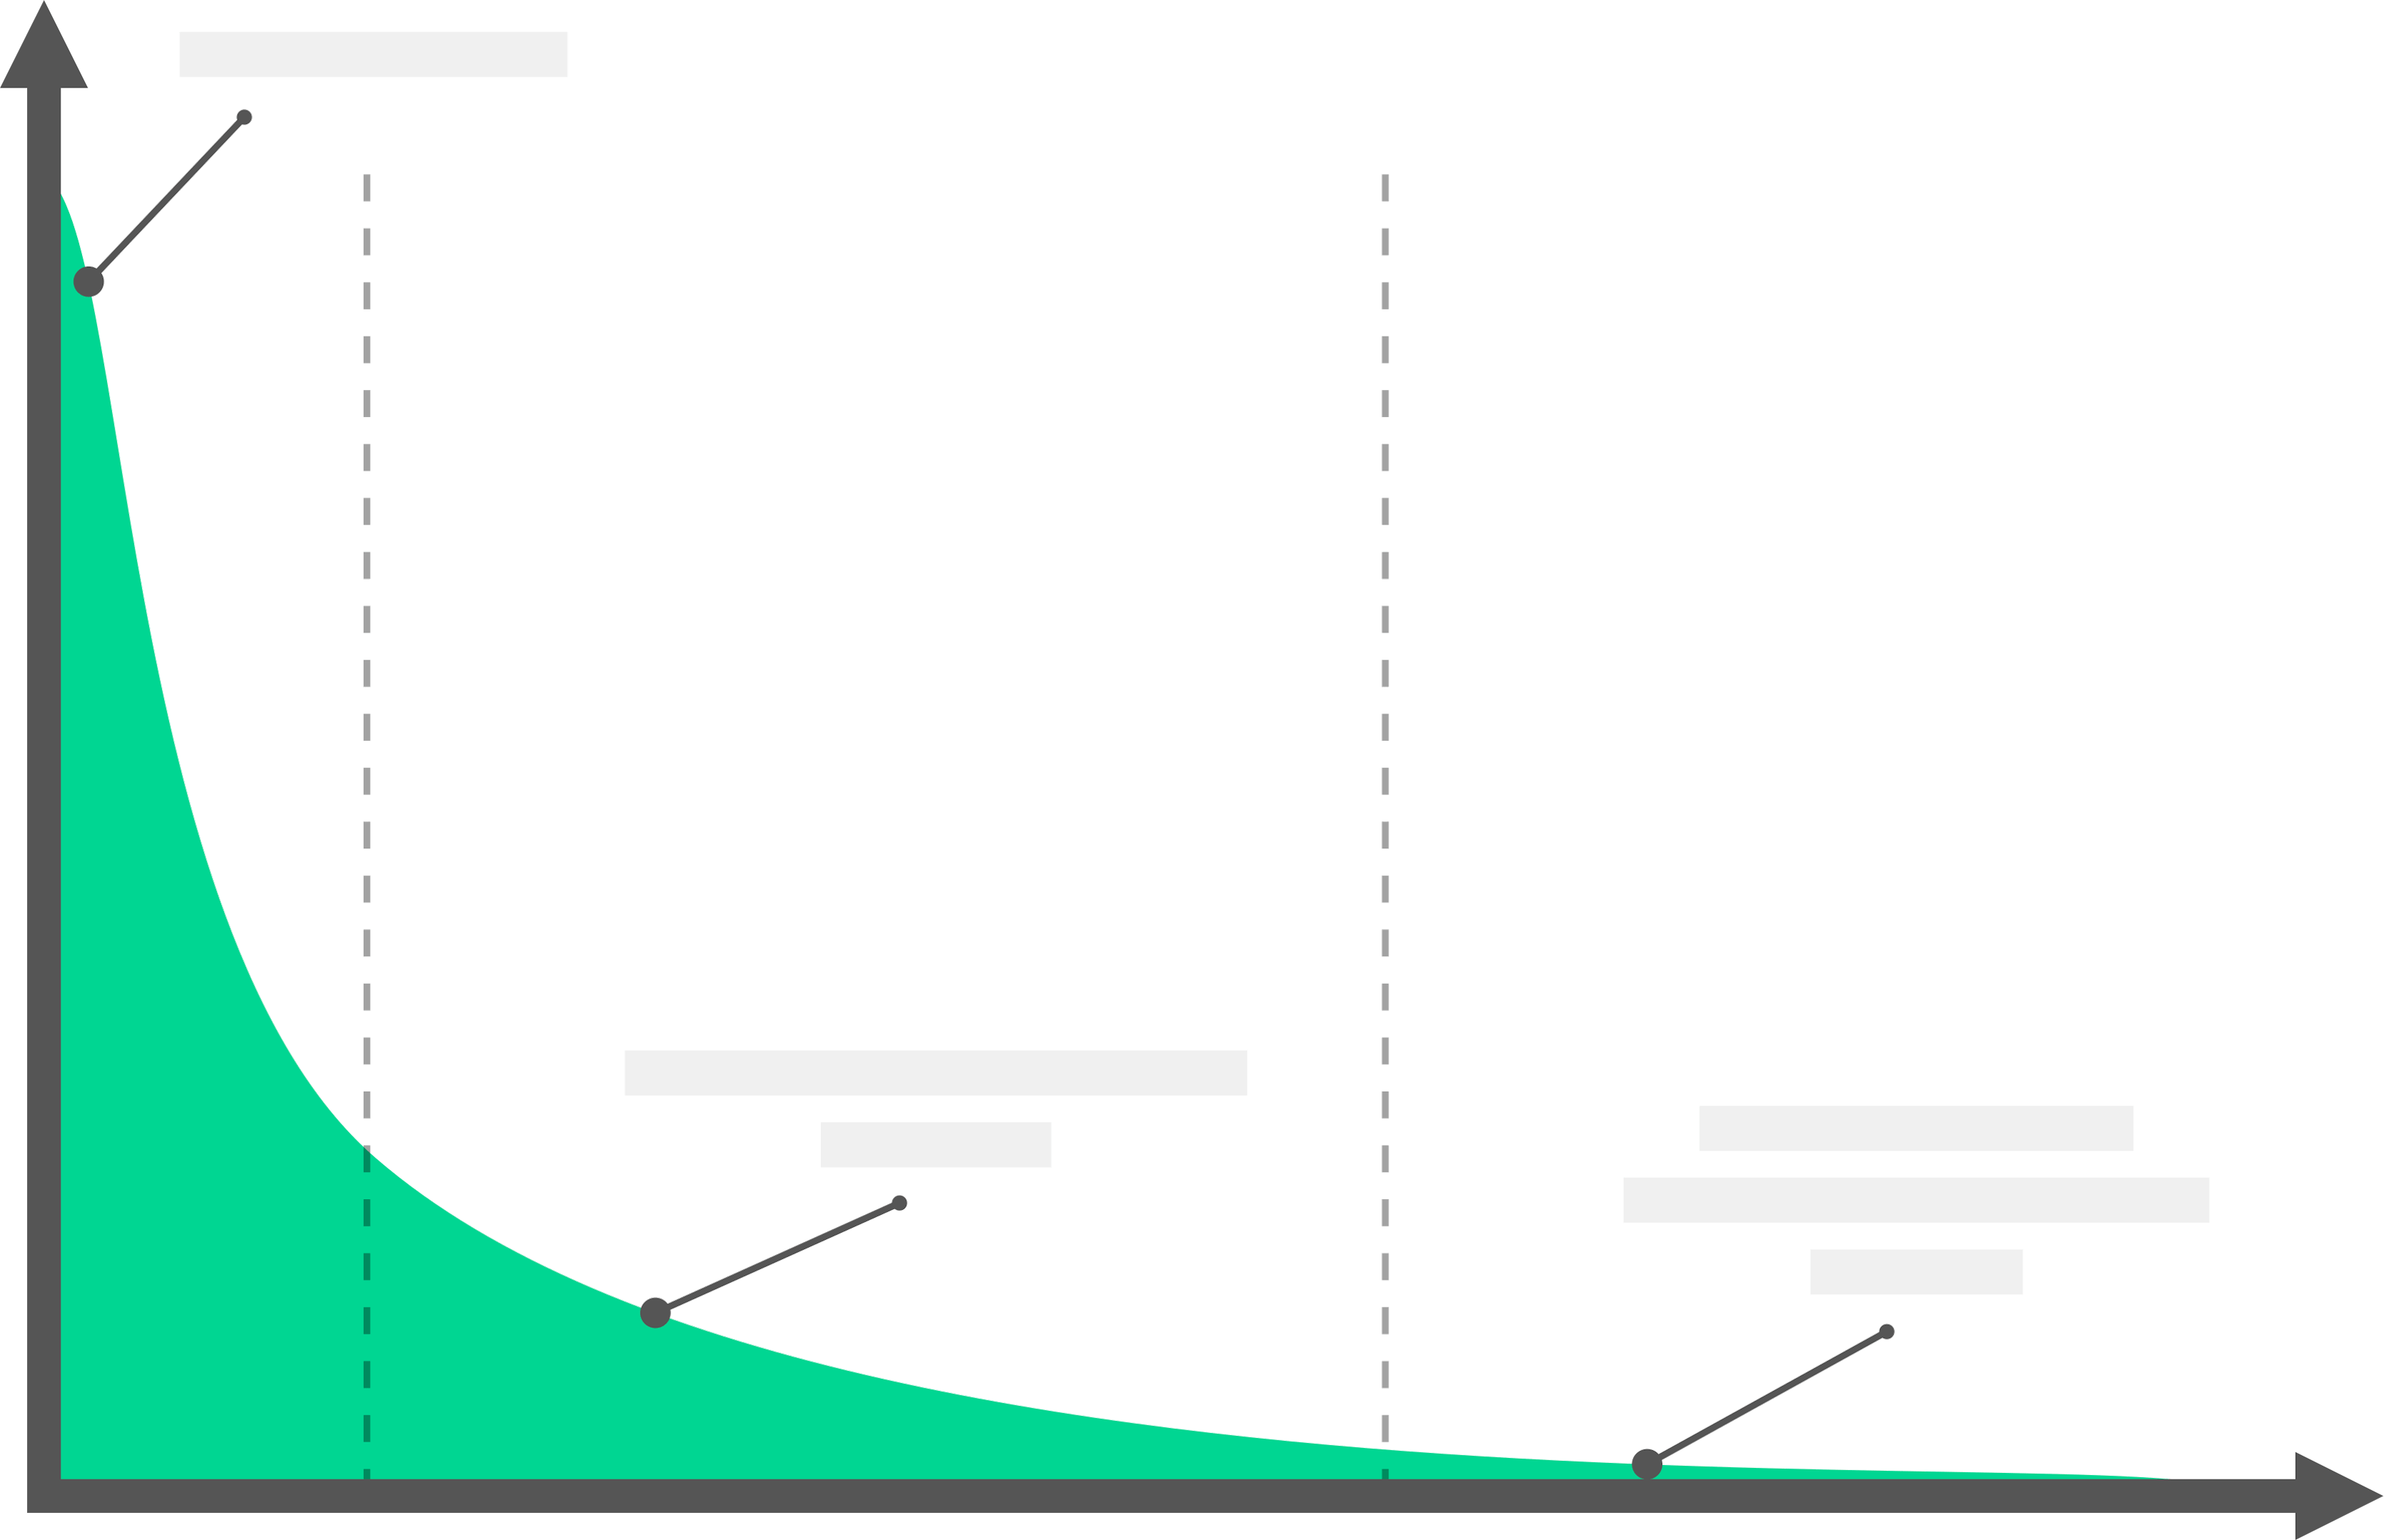
\includegraphics[width=0.7\linewidth]{FigureExample.png}
    % but in case of an svg file:
    %\includesvg[width=0.7\linewidth]{FigureExample.svg}
    \caption{Figure template}
    \label{fig:template}
\end{figure}





\section*{Table}

\begin{table}[H]
    \centering
    \caption{Table template}
    \label{tab:template}
    \begin{tabular}{|c|c|}
        \hline
        Cell A1 & Cell A2 \\
        \hline
        Cell B1 & Cell B2 \\
        \hline
    \end{tabular}
\end{table}





\section*{Mathematical formula}

\begin{equation}\label{eq:template}
a^2 + b^2 = c^3
\end{equation}
\eqcaption{Example Caption in List of Equations}




\section*{Listing}

\begin{lstlisting}[caption=Listing template, label=lst:template, language=Python]
print("Hello World!")
\end{lstlisting}